\begin{frame}
    \begin{center}
        \begin{tikzpicture}
            \node[anchor=south west,inner sep=0] (image) at (0,0) {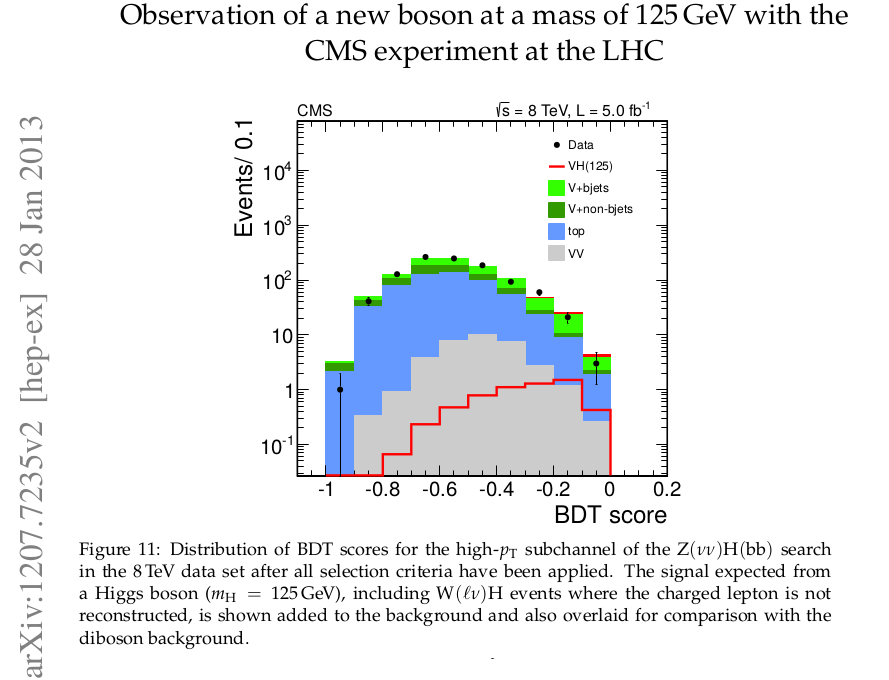
\includegraphics[width=0.8\textwidth]{higgs-cms-bdt.png}};
            \begin{scope}[x={(image.south east)},y={(image.north west)}]
                \onslide<2>{\draw[red, thick,rounded corners] (0.61,0.77) rectangle (0.7,0.74);}
                \onslide<2>{\draw[red, thick,rounded corners] (0.735,0.175) rectangle (0.805,0.145);}
                \onslide<3>{\draw[blue, thick,rounded corners] (0.61,0.74) rectangle (0.72,0.61);}
                \onslide<3>{\draw[blue, thick,rounded corners] (0.43,0.11) rectangle (0.55,0.08);}
            \end{scope}
        \end{tikzpicture}
    \end{center}
\end{frame}

\begin{frame}
    \begin{center}
        \begin{tikzpicture}
            \onslide<1>{\node[anchor=north west,inner sep=0] (image) at (0,0) {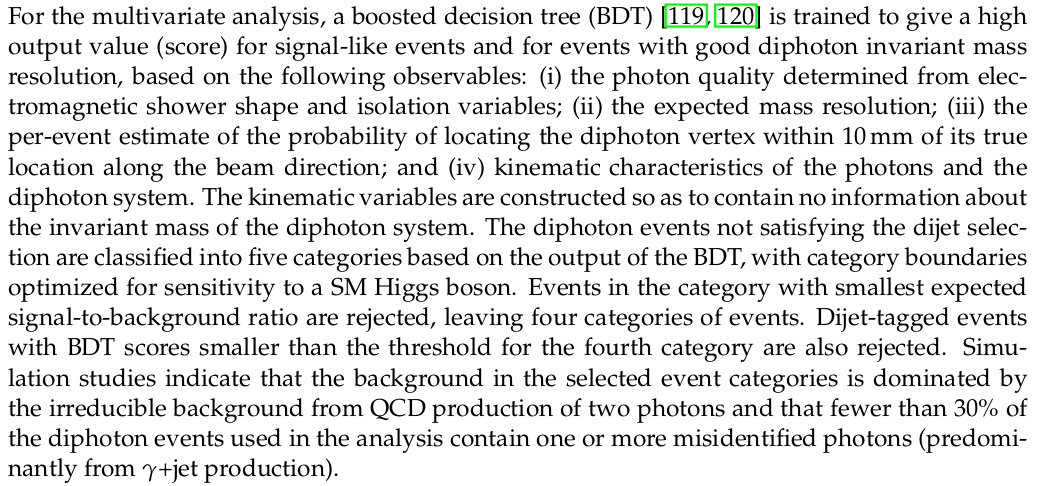
\includegraphics[width=\textwidth]{higgs-cms-bdt-text.png}};}
            \onslide<2->{\node[anchor=north west,inner sep=0] at (0,0) {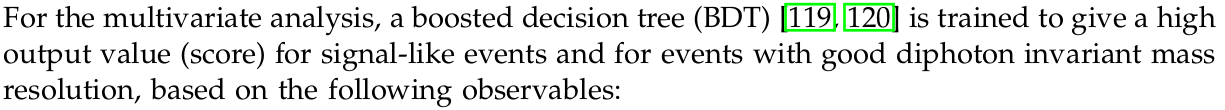
\includegraphics[width=\textwidth]{higgs-cms-bdt-text-important.png}};}
            \onslide<3>{\node[inner sep=0] at (2.4,-3.5) {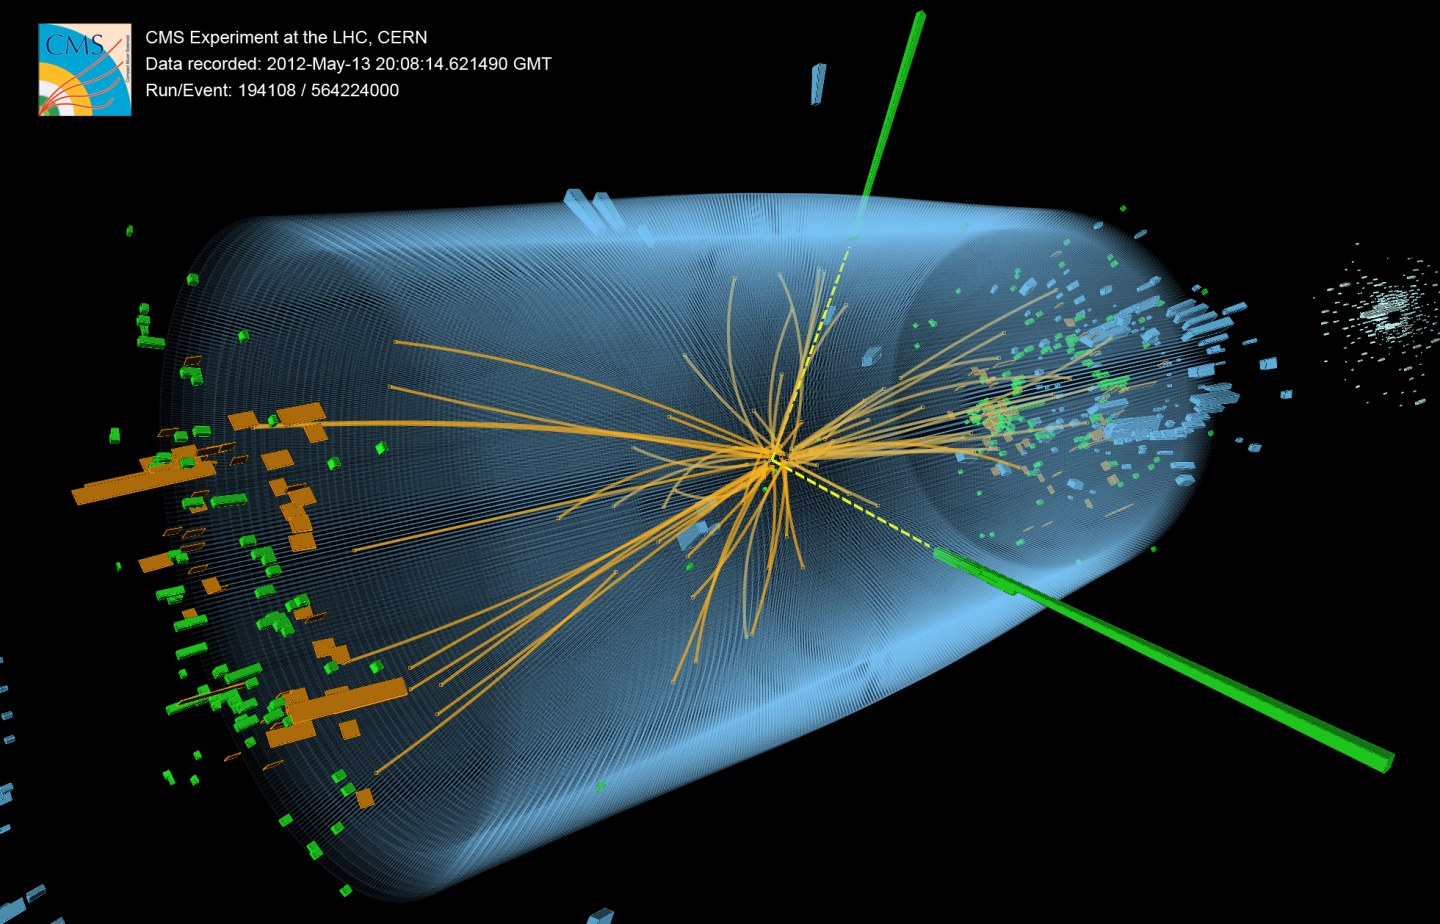
\includegraphics[width=0.4\textwidth]{higgs-cms-event.png}};}
            \onslide<3>{\node at (5.8,-3.5) [arrowstyle=2cm] {BDT};}
            \onslide<3>{\node[inner sep=0] at (9.3,-3.5) {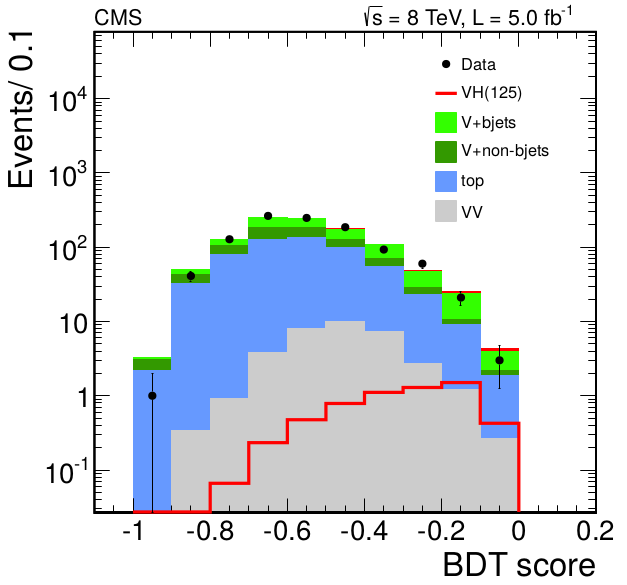
\includegraphics[width=0.4\textwidth]{higgs-cms-bdt-only.png}};}
        \end{tikzpicture}
    \end{center}
\end{frame}

\begin{frame}
  \frametitle{Outline}
  \vspace{-0.5cm}
  \begin{center}
  \begin{scriptsize}
    \tableofcontents[sectionstyle=show,subsectionstyle=show]
  \end{scriptsize}
  \end{center}
\end{frame}
